% ============================================================================
% AgriPerceiver -- ICA 2026 submission (Springer LNCS / CCIS format)
% Double-blind: author identity is withheld.
%
% Compilation (from paper-ica26/ directory):
%   pdflatex main
%   bibtex   main
%   pdflatex main
%   pdflatex main
%
% All required style files (llncs.cls, splncs04.bst) are included in this
% folder, so the project compiles directly on Overleaf with no extra setup.
% ============================================================================
\documentclass[runningheads]{llncs}

\usepackage[T1]{fontenc}
\usepackage{graphicx}
\usepackage{booktabs}
\usepackage{multirow}
\usepackage{amsmath,amssymb,mathtools}
\usepackage{enumitem}
\usepackage{float}
\usepackage{microtype}
\usepackage{listings}
\lstset{basicstyle=\ttfamily\footnotesize,breaklines=true,
        breakatwhitespace=true,frame=none,xleftmargin=0pt,
        columns=flexible,language={}}

% hyperref (loaded before cleveref); Springer eBook URL style
\usepackage{hyperref}
\renewcommand\UrlFont{\rmfamily}
\usepackage[capitalize]{cleveref}
% Springer-style cross-reference names
\crefname{figure}{Fig.}{Figs.}
\Crefname{figure}{Fig.}{Figs.}
\crefname{section}{Sect.}{Sects.}
\Crefname{section}{Sect.}{Sects.}
\crefname{equation}{Eq.}{Eqs.}
\Crefname{equation}{Eq.}{Eqs.}
\crefname{table}{Table}{Tables}
\Crefname{table}{Table}{Tables}

% Float tuning: help wide table floats stay near their reference
\setcounter{topnumber}{4}
\renewcommand{\topfraction}{0.95}
\renewcommand{\textfraction}{0.05}
\renewcommand{\floatpagefraction}{0.90}

% -- Macros -------------------------------------------------------------------
\newcommand{\ours}{AgriPerceiver}
\newcommand{\ie}{\textit{i.e.}}
\newcommand{\eg}{\textit{e.g.}}

\graphicspath{{figures/}}

\begin{document}

\title{AgriPerceiver: A Parameter-Efficient Vision-Language Model
for Structured Macroscopic Crop Phenotyping}
\titlerunning{AgriPerceiver: A Parameter-Efficient VLM for Crop Phenotyping}

% ---- Anonymised for double-blind review ------------------------------------
\author{Anonymous Author(s)}
\authorrunning{Anonymous Author(s)}
\institute{Affiliation withheld for double-blind review}

\maketitle

% ============================================================================
\begin{abstract}
Modern agriculture suffers from systemic crop yield instability, with plant pathogens contributing to 20--40\% of global yield losses. Adapting generalist Vision-Language Models (VLMs) to produce structured, actionable phenotyping from crop images creates a scalability crisis at the intersection of computer vision and agricultural life sciences. We present \textbf{\ours{}}, a lightweight VLM that frames this challenge as \emph{structured report generation}: given a single leaf photograph, the model produces a schema-compliant JSON diagnostic report detailing disease identity, pathology type, severity score, symptom characterisation, and actionable steps. To process high-resolution visual imagery, the input is spatially decomposed to preserve fine-grained pathological features that are typically lost during standard resizing. Our central contribution is a \emph{perception bridge} that mitigates visual token explosion by compressing visual tokens into just 128 learned latents ($28.5\times$ reduction) while critically preserving learned tile-position embeddings for spatial grounding. We employ a two-stage training curriculum: the bridge (${\sim}391$M parameters) is first aligned, followed by LoRA specialisation on Gemma-3-labelled structured annotations. Both the vision and language backbones remain strictly frozen throughout training to maintain parameter efficiency. Evaluated across nine metrics, AgriPerceiver achieves a composite score of \textbf{0.810} and 99.7\% schema compliance on a held-out test set, and improves pathology-type macro-F1 by $1.9\times$ over the strongest generalist baseline while training only $9.2\%$ of its parameters---demonstrating the viability of parameter-efficient domain specialisation in life-sciences AI for structured knowledge extraction.

\keywords{Vision-Language Models \and Agricultural Pathology \and Perceiver Resampler \and Life Sciences AI \and LoRA \and Structured Output Generation}
\end{abstract}

% ============================================================================
\section{Introduction}
\label{sec:intro}

Pathogen-induced crop losses account for 20--40\% of global agricultural output annually~\cite{savary2019global}, making plant disease diagnosis one of the highest-impact problems in life sciences and food security. Conventional diagnostic workflows require trained agronomists to inspect
field samples and produce structured reports that cover disease type, severity, observed symptoms, and treatment recommendations, making it a slow and resource-intensive process that cannot scale to the hundreds of millions of smallholder farms that most need it. We frame this problem through the lens of life-sciences AI, making it a multi-modal grounding problem: macroscopic visual phenotypes must be mapped to a
structured biological ontology, pathogen taxonomy, severity index and therapeutic action---the same integration that generalises across both macroscopic and microscopic scales.

Vision-language models (VLMs) offer a principled path toward automating
this diagnosis, yet adaptation of a general-purpose VLM into agricultural pathology exposes three fundamental limitations.
\emph{First}, standard visual token budgets are designed for natural images, not the high-resolution, fine-grained symptom patterns (\ie{} fungal lesions, bacterial water-soaking and nutrient-deficiency chlorosis) that distinguish disease classes at the microscopic scale. Naively increasing the token budget to preserve these details incurs a quadratic attention cost that quickly exceeds commodity hardware. \emph{Second}, autoregressive VLM output is free-form text, incompatible with the structured JSON schemas required by agricultural decision-support APIs. \emph{Third}, state-of-the-art VLMs are generalist and carry billions of parameters
trained on web-scale corpora and cannot be specialised affordably on low-compute infrastructure.

We address these limitations with \textbf{\ours{}}, contributing:

\begin{enumerate}[leftmargin=*,topsep=2pt,itemsep=2pt]
  \item A \emph{perception bridge}: AnyRes spatial tiling, learned
        tile-position embeddings, an MLP projector, and a two-block \textbf{Perceiver Resampler} that compresses 3,645 visual tokens into 128 latents ($28.5\times$), reducing per-layer attention cost by $27.5\times$ (\cref{sec:complexity}) while retaining spatial fidelity for microscopic symptom analysis.

  \item A \emph{two-stage training curriculum}: \textbf{bridge-only alignment
        pretraining} followed by LoRA-based specialisation, keeping both
        frozen backbones (${\sim}4.22$B parameters) out of the gradient
        path, so only ${\sim}426$M parameters (${\sim}9.2\%$ of 4.6B) are
        updated in Stage~2.

  \item An \emph{automated data pipeline and rigorous evaluation framework}:
        we leverage Gemma-3-12B-IT~\cite{gemmateam2025gemma3} to label 117K agricultural
        images into a schema-compliant, seven-field JSON format. Model assessment is then
        conducted across a comprehensive nine-metric suite covering five distinct quality dimensions, together with a per-class, calibration, and complexity analysis.
\end{enumerate}

Across all five evaluation axes, \ours{} attains a composite score of $0.810$ versus $0.615$ for the strongest generalist baseline, a $1.9\times$ improvement in pathology-type macro-F1 over the strongest baseline (up to $4.8\times$ over the weakest), and a $3.3\times$ reduction in severity error, while remaining trainable on a single GPU.

% ============================================================================
\section{Related Work}
\label{sec:related}

\subsection{Vision-Language Models and Structured Output}
Generalist VLMs such as LLaVA~\cite{liu2024visual}, InternVL~\cite{chen2024internvl}, and Qwen2-VL~\cite{wang2024qwen2vl} couple a frozen vision encoder to a large language model through a lightweight connector, and demonstrate strong capabilities in visual question answering and image captioning. Their training objective, however, optimises free-form conversational text; when prompted for machine-readable output they produce syntactically valid but semantically shallow structures, as our experiments confirm (\cref{sec:main}). Adapting these architectures to reliable structured scientific output---where a downstream API consumes a fixed schema---remains an open challenge that prompt engineering alone does not solve. \ours{} instead treats the schema as a first-class training target, specialising a compact backbone so that structural compliance and field-level accuracy are learned jointly.

\subsection{Visual Token Compression}
The number of visual tokens a VLM must process grows with input resolution, and self-attention over these tokens scales quadratically, creating a memory and compute bottleneck for high-resolution scientific imagery. The Perceiver~\cite{jaegle2021perceiver} and Flamingo's Perceiver Resampler~\cite{alayrac2022flamingo} address this by introducing a small set of learned latent queries that cross-attend to the full visual sequence, decoupling downstream cost from input length. Recent VLMs (\eg{} InternVL) instead employ dynamic high-resolution tiling for general scenes. \ours{} combines both ideas but adapts them to pathology: it tiles at high resolution to expose microscopic lesions, then compresses aggressively through a Perceiver Resampler, while injecting learned tile-position embeddings so that spatial provenance survives compression---a property we show aids free-text localisation of symptoms (\cref{sec:ablation}).

\subsection{Parameter-Efficient Adaptation}
Full fine-tuning of multi-billion-parameter backbones is prohibitively expensive and risks catastrophic forgetting of pretrained knowledge. Parameter-efficient fine-tuning, most prominently LoRA~\cite{hu2022lora}, injects low-rank update matrices into frozen weights, updating a small fraction of parameters. Quantised variants such as QLoRA~\cite{dettmers2024qlora} further reduce the memory footprint of both training and the teacher models used for annotation. \ours{} pushes this paradigm to its limit for the structured-generation setting: both the SigLIP~\cite{zhai2023sigmoid} vision encoder and the Phi-3-mini~\cite{abdin2024phi3} language model remain strictly frozen, and only the perception bridge and rank-32 LoRA adapters---together $9.2\%$ of the system---receive gradients.

\subsection{AI for Agricultural Pathology}
In agricultural AI, PlantVillage~\cite{mohanty2016using} established the foundation for deep-learning disease classification, though its legacy relies primarily on scalar, single-label predictions over curated, controlled-background imagery. Domain-specialised multimodal pretraining has proven effective at molecular and clinical scales---for example BiomedCLIP~\cite{zhang2023biomedclip}---yet macroscopic agricultural pathology remains comparatively underserved. Transitioning from single-label classification to rich, multi-dimensional diagnostic reporting (identity, type, severity, symptoms, reasoning, and actions) requires processing high-resolution imagery under tight compute constraints and emitting a structured report rather than a class index. \ours{} targets exactly this gap.

% ============================================================================
\section{Problem Formulation}
\label{sec:problem}

We cast macroscopic crop phenotyping as \emph{conditional structured sequence generation}. Given a single leaf image $I \in \mathbb{R}^{H \times W \times 3}$ of arbitrary resolution and a fixed instruction prompt $\mathbf{x}_{\text{txt}}$, the model must produce a token sequence $\mathbf{y} = (y_1,\ldots,y_L)$ that deserialises into a JSON object $R$ conforming to a fixed seven-field schema $\mathcal{S}$:
\begin{equation}
  R = \{\,\text{diagnosis},\, \text{type},\, \text{severity},\, \text{confidence},\, \text{symptoms},\, \text{reasoning},\, \text{actions}\,\}.
  \label{eq:schema}
\end{equation}
Here $\text{type}\in\mathcal{T}$ is a categorical pathology label over $|\mathcal{T}|{=}6$ classes, $\text{severity},\text{confidence}\in[0,1]$ are continuous, and the remaining fields are free-form natural language. Let $f_\phi$ denote the frozen vision encoder, $g_\theta$ the trainable perception bridge, and $p_\psi$ the language model with LoRA parameters $\psi$. The model factorises the report autoregressively,
\begin{equation}
  p(\mathbf{y}\mid I, \mathbf{x}_{\text{txt}})
  = \prod_{t=1}^{L} p_\psi\!\bigl(y_t \mid y_{<t},\, g_\theta(f_\phi(I)),\, \mathbf{x}_{\text{txt}}\bigr),
  \label{eq:factorization}
\end{equation}
and is trained to maximise the likelihood of teacher-provided reference reports. A prediction is deemed \emph{schema-compliant} if $\mathbf{y}$ parses as valid JSON and instantiates all seven fields of $\mathcal{S}$ with type-correct values. This formulation unifies classification (the \text{type} field), regression (\text{severity}), and language generation (\text{symptoms}, \text{reasoning}, \text{actions}) under a single decoding objective, and motivates the multi-axis evaluation of \cref{sec:eval}.

% ============================================================================
\section{Method}
\label{sec:method}

\subsection{Architecture Overview}

\ours{} (\cref{fig:architecture}) processes an input leaf image through
four sequential stages:
(1)~a frozen SigLIP-SO400M~\cite{zhai2023sigmoid} vision encoder,
(2)~a trainable \emph{perception bridge} (TileEmbeddings $\to$
VisionProjector $\to$ PerceiverResampler),
(3)~a splice-and-forward multimodal fusion mechanism, and
(4)~a Phi-3-mini-128k~\cite{abdin2024phi3} language model with LoRA
adapters in Stage~2. Phi-3-mini's 128K context window accommodates long structured JSON
outputs without truncation; its compact 3.8B parameter footprint keeps
the full inference stack within a single-GPU 24\,GB VRAM budget.

\begin{figure}[t]
  \centering
  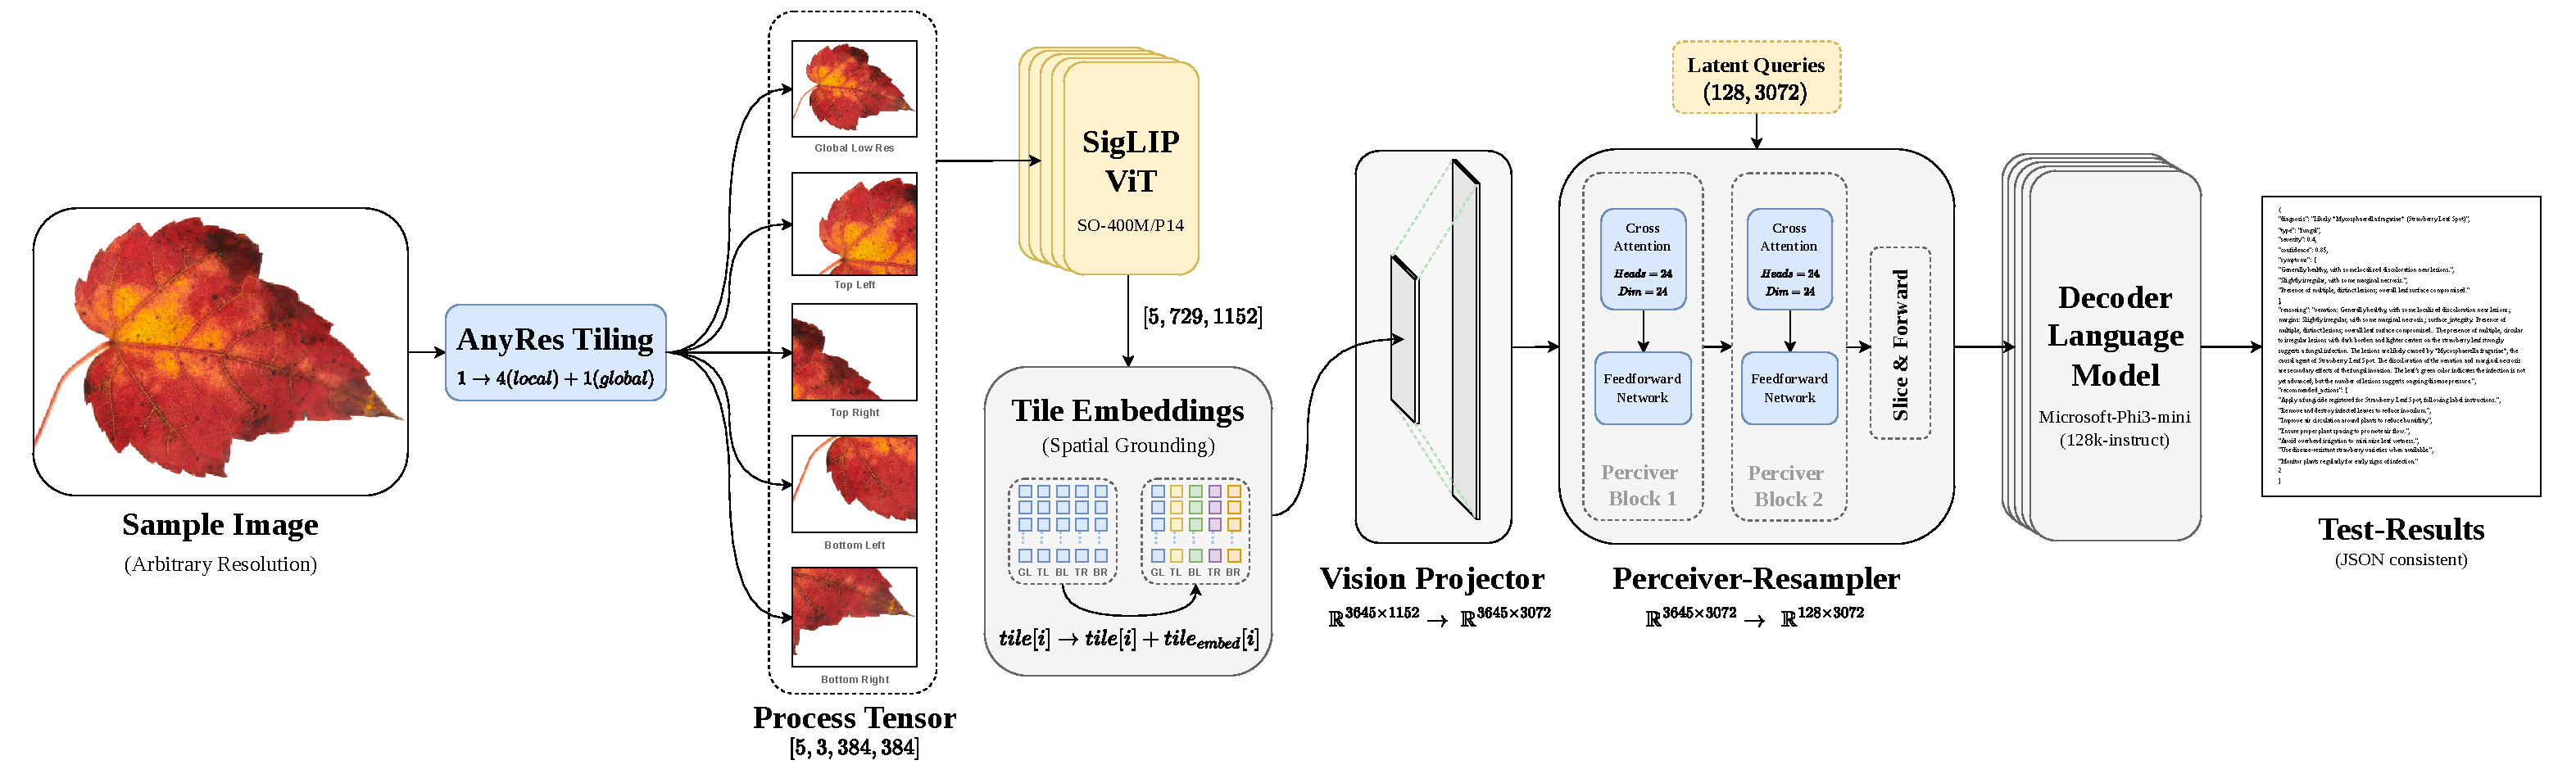
\includegraphics[width=\textwidth]{architecture.pdf}
  \caption{\textbf{\ours{} architecture.}
  \textbf{(1) Tiling:} the input is decomposed into 5 AnyRes tiles, capturing both global context and fine-grained local details at ${\approx}2\times$ effective resolution.
  \textbf{(2) Encoding:} a frozen SigLIP extracts patch tokens, which are enriched with learned spatial embeddings.
  \textbf{(3) Compression:} a two-block Perceiver Resampler compresses the visual sequence ($28.5\times$ reduction, from 3,645 to 128 latents).
  \textbf{(4) Generation:} these latents are spliced into a frozen Phi-3-mini to drive autoregressive structured JSON generation.}
  \label{fig:architecture}
\end{figure}

\subsection{AnyRes Spatial Tiling}

Each input image $I \in \mathbb{R}^{H \times W \times 3}$, regardless
of native resolution, is decomposed into five tiles: four equal quadrant
crops (top-left, top-right, bottom-left, bottom-right) and one globally
resized view, each rescaled to $384 \times 384$.
The tile tensor $\mathbf{T} \in \mathbb{R}^{5 \times 3 \times 384 \times
384}$ is processed in parallel by SigLIP, yielding patch features
$\mathbf{V} \in \mathbb{R}^{5 \times 729 \times 1152}$
($729 = 27 {\times} 27$ patches per tile, $d_v = 1152$).
Quadrant crops provide approximately $2\times$ effective resolution for
fine-grained lesion analysis; the global tile preserves holistic leaf
context.

\subsection{Perception Bridge}

\paragraph{Tile Embeddings.}
A learned parameter matrix $\mathbf{E} \in \mathbb{R}^{5 \times 1152}$
assigns each tile a distinct spatial identity.
For tile $t$, embedding $\mathbf{e}_t$ is broadcast and added to all 729
patch tokens:
\begin{equation}
  \widetilde{\mathbf{V}}_{t,p} = \mathbf{V}_{t,p} + \mathbf{e}_t,
  \quad t \in \{1,\ldots,5\},\; p \in \{1,\ldots,729\}.
  \label{eq:tile_embed}
\end{equation}
This encoding enables the downstream modules to recover the spatial
origin of each patch without modifying the frozen encoder.

\paragraph{Vision Projector.}
The enriched features are reshaped to
$\widetilde{\mathbf{V}} \in \mathbb{R}^{3645 \times 1152}$
($3645 = 5 \times 729$) and projected into the LLM dimension $d_l =
3072$ via a two-layer MLP with GELU activation:
\begin{equation}
  \mathbf{V}' = \mathrm{MLP}_\theta(\widetilde{\mathbf{V}})
  \in \mathbb{R}^{3645 \times 3072}.
  \label{eq:projector}
\end{equation}

\paragraph{Perceiver Resampler.}
A set of $N = 128$ learned latent queries
$\mathbf{Q} \in \mathbb{R}^{128 \times 3072}$
iteratively attend to $\mathbf{V}'$ through $D = 2$ PerceiverBlocks.
Each block applies scaled dot-product attention
\begin{equation}
  \mathrm{Attn}(\mathbf{Q},\mathbf{K},\mathbf{V})
    = \mathrm{softmax}\!\Bigl(\tfrac{\mathbf{Q}\mathbf{K}^{\!\top}}{\sqrt{d_h}}\Bigr)\mathbf{V},
    \qquad d_h = d_l / H,
  \label{eq:attn}
\end{equation}
in a cross-attention, self-attention, feed-forward sequence with RMSNorm and residual connections:
\begin{align}
  \mathbf{Z}^{(d)} &= \mathbf{Z}^{(d-1)}
    + \mathrm{CrossAttn}\!\left(\mathrm{RMSNorm}(\mathbf{Z}^{(d-1)}),\,
    \mathbf{V}'\right), \notag\\
  \mathbf{Z}^{(d)} &= \mathbf{Z}^{(d)}
    + \mathrm{SelfAttn}\!\left(\mathrm{RMSNorm}(\mathbf{Z}^{(d)})\right),
    \notag\\
  \mathbf{Z}^{(d)} &= \mathbf{Z}^{(d)}
    + \mathrm{GLU\text{-}FFN}\!\left(\mathrm{RMSNorm}(\mathbf{Z}^{(d)})\right),
  \label{eq:perceiver}
\end{align}
with $H = 24$ attention heads, where in the cross-attention the queries derive from the latents $\mathbf{Z}$ and the keys/values from the visual features $\mathbf{V}'$. The GLU-FFN is a gated linear unit, $\mathrm{GLU\text{-}FFN}(\mathbf{u}) = \bigl(\mathrm{GELU}(\mathbf{u}\mathbf{W}_g)\odot \mathbf{u}\mathbf{W}_v\bigr)\mathbf{W}_o$ with a $4\times$ hidden expansion.
Initialising $\mathbf{Z}^{(0)} = \mathbf{Q}$, the final output
$\mathbf{Z} \in \mathbb{R}^{128 \times 3072}$ achieves $3{,}645 \to 128$
token compression ($28.5\times$) with no reduction in the capacity
available to the downstream LLM.

\subsection{Splice-and-Forward Fusion}

The 128 compressed latents replace the \texttt{<image>} placeholder
in the text prompt:
\begin{equation}
  \mathbf{X} = \bigl[\mathbf{x}_{\text{pre}};
  \underbrace{\mathbf{Z}}_{128\,\text{tokens}};
  \mathbf{x}_{\text{post}}\bigr],
  \label{eq:splice}
\end{equation}
where $\mathbf{Z}$ acts as the visual prompt representation. Phi-3's causal transformer then processes this hybrid sequence with \texttt{use\_cache=False}.

\subsection{Two-Stage Training Curriculum}

\subsubsection{Stage 1 --- Alignment.}
Only the perception bridge (${\sim}391$M parameters:
TileEmbeddings + VisionProjector + PerceiverResampler; see \cref{app:params}) is trained
on generic image--caption pairs from 117K agricultural images using
standard causal LM cross-entropy loss.
Both SigLIP and Phi-3 are frozen throughout.
Training runs for 2 epochs (14.7K gradient steps) with batch size 16,
learning rate $10^{-4}$ (AdamW), and bfloat16 precision.

\subsubsection{Stage 2 --- Specialisation.}
LoRA adapters ($r{=}32$, $\alpha{=}64$, dropout $0.1$) are attached to
Phi-3's \texttt{qkv\_proj}, \texttt{o\_proj}, \texttt{gate\_up\_proj},
\texttt{down\_proj}, and \texttt{up\_proj} modules (${\sim}35$M
parameters).
The bridge and LoRA (${\sim}426$M total, ${\approx}9.2\%$ of the 4.6B
system) are jointly fine-tuned on 96,239 structured JSON samples for 3 epochs
(37.9K steps, batch size 8, gradient accumulation $k{=}2$) using a
per-sample weighted cross-entropy objective:
\begin{equation}
  \mathcal{L} =
  \frac{1}{|B|} \sum_{i \in B}\, w_i \cdot
  \mathrm{CE}(\hat{\mathbf{y}}_i,\, \mathbf{y}_i),
  \label{eq:loss}
\end{equation}
where $w_i \in [0,1]$ is derived from Gemma-3's per-sample generation
confidence, providing a curriculum effect that up-weights
high-confidence structured labels.

\subsection{Attention Complexity Analysis}
\label{sec:complexity}

The primary motivation for the Perceiver Resampler is to decouple attention cost from input resolution, which is non-negotiable when microscopic fungal hyphae or bacterial pustules must remain resolvable. Let $T_v$ be the number of visual tokens, $N$ the number of latents, and $d$ the model width. Standard self-attention over the full sequence forms an $T_v \times T_v$ attention map and costs
\begin{equation}
  \mathcal{F}_{\text{full}} = 4\,T_v^2\,d
  \quad\text{(FLOPs per layer, projections excluded),}
  \label{eq:full}
\end{equation}
scaling \emph{quadratically} in $T_v$. The Perceiver instead lets $N$ latents cross-attend to the $T_v$ tokens and then self-attend among themselves,
\begin{equation}
  \mathcal{F}_{\text{perc}} = \underbrace{4\,N\,T_v\,d}_{\text{cross-attn}}
  \; + \; \underbrace{4\,N^2\,d}_{\text{latent self-attn}},
  \label{eq:perc}
\end{equation}
which is \emph{linear} in $T_v$. For our configuration ($T_v{=}3{,}645$, $N{=}128$, $d{=}3072$), this yields $\mathcal{F}_{\text{full}}{=}163.3$\,GFLOP versus $\mathcal{F}_{\text{perc}}{=}5.93$\,GFLOP per layer---a $27.5\times$ reduction (\cref{tab:complexity})---and shrinks the per-head attention map from $13.29$M to $0.47$M entries. \Cref{fig:flops} shows that the gap widens with each additional tile: because the latent count is fixed, the 128 latents furnish a constant-size ``visual summary'' whose downstream cost is invariant to how many AnyRes tiles we add, ensuring predictable inference latency as resolution scales.

\begin{table}[t]
  \centering
  \caption{Attention cost per layer, full self-attention over the visual
    sequence versus the Perceiver Resampler, at the deployed configuration
    ($T_v{=}3{,}645$ tokens, $N{=}128$ latents, $d{=}3072$).
    FLOPs from \cref{eq:full,eq:perc}; projection terms excluded for both.}
  \label{tab:complexity}
  \setlength{\tabcolsep}{8pt}
  \begin{tabular}{@{}lccc@{}}
    \toprule
    & \textbf{Full self-attn.} & \textbf{Perceiver} & \textbf{Reduction} \\
    \midrule
    Attention scaling            & $O(T_v^2 d)$ & $O(N T_v d)$ & --- \\
    Attn.\ map / head (entries)  & 13.29\,M     & 0.47\,M      & $28.5\times$ \\
    Attn.\ FLOPs / layer         & 163.3\,G     & 5.93\,G      & $27.5\times$ \\
    Downstream visual tokens     & 3{,}645      & 128          & $28.5\times$ \\
    \bottomrule
  \end{tabular}
\end{table}

\begin{figure}[t]
  \centering
  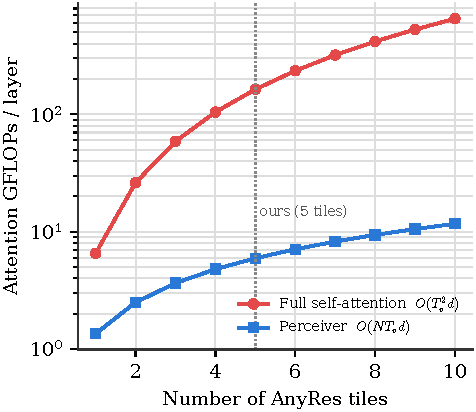
\includegraphics[width=0.62\textwidth]{flops.pdf}
  \caption{Per-layer attention FLOPs as a function of the number of AnyRes
    tiles (log scale). Full self-attention grows quadratically with the visual
    sequence length $T_v$; the Perceiver Resampler grows linearly, because the
    128 latents cross-attend to $T_v$ tokens and then self-attend at fixed cost.
    The dotted line marks our deployed 5-tile configuration.}
  \label{fig:flops}
\end{figure}

% ============================================================================
\section{Automated Data Pipeline}
\label{sec:data}

We curate 117,635 agricultural leaf images and generate structured labels
using Gemma-3-12B-IT~\cite{gemmateam2025gemma3} operating under 4-bit NF4
quantisation~\cite{dettmers2024qlora} with an eight-shot structured-JSON exemplar prompt.
Each label encodes the seven-field JSON schema of \cref{eq:schema}: \emph{diagnosis}, \emph{type}
(fungal/bacterial/viral/pest/deficiency/unknown), \emph{severity}~$\in[0,1]$,
\emph{confidence}~$\in[0,1]$, \emph{symptoms}, \emph{reasoning}, and
\emph{recommended\_actions} (see \cref{app:schema} for a full example).

Crucially, to ensure dataset quality, generation confidence is derived directly from
Gemma-3's output-token transition probabilities (the geometric mean of
$\exp(\text{transition\_score})$). This provides a calibrated signal grounded in the
model's inherent generative uncertainty, entirely bypassing the unreliability of its
self-reported \texttt{confidence} field.

Applying a strict filtering threshold based on this metric ($\tau{=}0.5$),
101,301 samples (86\%) pass our quality checks, yielding 96,239 training instances
and a 5,062-sample held-out test set. The training samples are stratified
into easy, medium, and hard curriculum buckets (\cref{app:datapipeline}), which explicitly dictate the
per-sample training weight $w_i$ applied in \cref{eq:loss}; the class balance of the
resulting test set is reported in \cref{app:datapipeline}.

% ============================================================================
\section{Experiments}
\label{sec:exp}

\subsection{Evaluation Framework}
\label{sec:eval}

We measure model quality along nine metrics across five axes.
\textbf{Structural}: JSON validity (\%) and schema compliance (\%).
\textbf{Classification}: pathology-type macro-F1 and diagnosis
fuzzy-match. Macro-F1 averages the per-class F1 uniformly,
\begin{equation}
  F_1^{\text{type}} = \frac{1}{|\mathcal{T}|}\sum_{c\in\mathcal{T}}
  \frac{2\,P_c R_c}{P_c + R_c},
  \label{eq:macrof1}
\end{equation}
so that rare classes count equally. Diagnosis fuzzy-match uses a token-Jaccard
criterion: for predicted and reference name token sets $A,B$, the sample counts
as correct when $J(A,B)=|A\cap B|/|A\cup B|\ge 0.6$.
\textbf{Regression}: severity mean absolute error (MAE) and Pearson $r$.
\textbf{Semantic}: BERTScore F1~\cite{zhang2020bertscore} for the
symptoms, reasoning, and recommended-actions fields.
\textbf{Calibration}: Expected Calibration Error (ECE, 10 bins,
lower is better; defined in \cref{app:calibration}).
These are aggregated into a single composite score:
\begin{align}
  \mathcal{C} =&\; 0.20\,F_1^{\text{type}}
    + 0.15\,F_{\text{diag}}
    + 0.15\,B_{\text{sym}}
    + 0.10\,(1 - \mathrm{MAE}) \notag\\
    &+ 0.10\,B_{\text{reas}}
    + 0.10\,B_{\text{act}}
    + 0.10\,J_{\text{val}}
    + 0.05\,(1 - \mathrm{ECE}) \notag\\
    &+ 0.05\,S_{\text{cmp}},
  \label{eq:composite}
\end{align}
where $B_{\cdot}$ are BERTScore F1 values, $J_{\text{val}}$ is JSON
validity, and $S_{\text{cmp}}$ is schema compliance; all components
lie in $[0,1]$ (higher is better). The weighting places the highest single weight on
pathology type---the primary agronomic decision signal---while the three semantic
BERTScore terms collectively receive the largest share ($0.35$), reflecting the
report's role as a human-facing document. \Cref{app:composite} verifies that the
system ranking is invariant to substantial reweighting.

\subsection{Main Results}
\label{sec:main}

\begin{table}[t]
  \centering
  \caption{Main results on the 5,062-sample held-out test set.
    $\downarrow$: lower is better.
    \ours{} (4.6B) trains only bridge+LoRA (${\sim}426$M, $9.2\%$);
    both backbones frozen.
    BERT-F1: symptom BERTScore F1.}
  \label{tab:main}
  \setlength{\tabcolsep}{5pt}
  \resizebox{\textwidth}{!}{%
  \begin{tabular}{@{}l cc cc cc c c@{}}
    \toprule
    \multirow{2}{*}{\textbf{Model}}
      & \multicolumn{2}{c}{\textbf{Structural}}
      & \multicolumn{2}{c}{\textbf{Classification}}
      & \multicolumn{2}{c}{\textbf{Regression}}
      & \textbf{Semantic}
      & \multirow{2}{*}{\textbf{Composite}} \\
    \cmidrule(lr){2-3}\cmidrule(lr){4-5}\cmidrule(lr){6-7}\cmidrule(lr){8-8}
      & JSON\% & Schema\%
      & Type-F1 & Diag-FM
      & MAE$\downarrow$ & Pearson $r$
      & BERT-F1 & \\
    \midrule
    LLaVA-NeXT-7B~\cite{liu2024llavanext}
      & 99.9 & 99.9 & 0.134 & 0.001 & 0.344 & 0.226 & 0.847 & 0.590 \\
    InternVL2-8B~\cite{chen2024internvl}
      & 100.0 & 100.0 & 0.336 & 0.005 & 0.385 & 0.624 & 0.848 & 0.611 \\
    Qwen2-VL-7B~\cite{wang2024qwen2vl}
      & 99.9 & 99.9 & 0.287 & 0.001 & 0.224 & 0.666 & 0.830 & 0.615 \\
    \midrule
    \textbf{\ours{} (ours)}
      & 99.7 & 99.7
      & \textbf{0.645} & \textbf{0.486}
      & \textbf{0.067} & \textbf{0.855}
      & \textbf{0.921} & \textbf{0.810} \\
    \bottomrule
  \end{tabular}}
\end{table}

\Cref{tab:main} compares \ours{} against three general-purpose VLMs
of comparable or larger scale on the 5,062-sample held-out test set. All baselines receive the identical structured-JSON system prompt and are evaluated with the same metric pipeline. \ours{} achieves near-perfect structural compliance (99.7\%).
Severity regression yields Pearson $r = 0.855$ and MAE $= 0.067$ on
the $[0,1]$ scale (RMSE $=0.125$)---both within useful bounds for
severity triage, and $3.3\times$ lower MAE than the best baseline
(Qwen2-VL-7B; MAE $= 0.224$).
Pathology-type macro-F1 of 0.645 is $1.9\times$ the best generalist baseline
(InternVL2, 0.336) and $4.8\times$ the weakest (LLaVA-NeXT, 0.134). The overall
composite of 0.810 exceeds the strongest baseline (Qwen2-VL, 0.615) by $+0.195$ (${+}32\%$).
Baselines exhibit near-total failure on bacterial (F1 $\leq 0.025$),
pest (F1 $\leq 0.017$), and viral (F1 $\leq 0.022$) classes, and
LLaVA-NeXT collapses to predicting ``unknown'' for 98.7\% of samples---a
degenerate strategy examined further in \cref{sec:perclass}.

\subsection{Per-Class Analysis}
\label{sec:perclass}

\Cref{fig:perclass} decomposes pathology-type F1 by class. The generalist
baselines are competitive only on \emph{fungal} and \emph{unknown}---the two
largest and most visually distinctive classes---and collapse to near-zero F1 on
bacterial, pest, and viral pathologies, whose discriminative cues (leaf-margin
water-soaking, pest frass, viral mosaic) are subtle and not salient under generic
visual prompting. \ours{} is the only model that produces usable predictions
across all six classes, lifting the three hardest classes from $\leq 0.025$ to
$0.525$--$0.560$.

\begin{figure}[t]
  \centering
  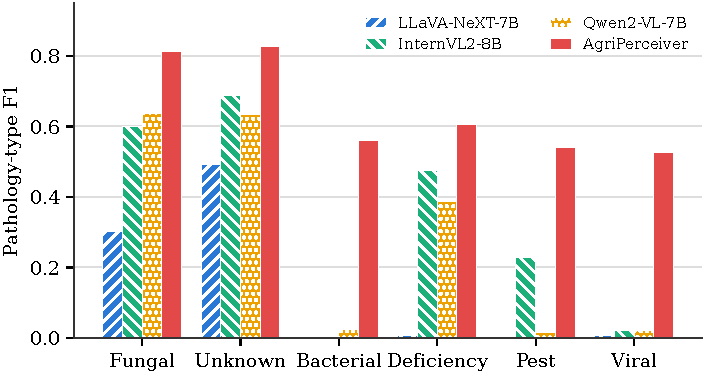
\includegraphics[width=0.92\textwidth]{perclass_f1.pdf}
  \caption{Per-class pathology-type F1 on the held-out test set. Generalist
    baselines succeed only on the large, visually distinctive fungal and unknown
    classes and collapse on bacterial, pest, and viral pathologies; \ours{} (red)
    is the only model usable across all six classes. Baseline values follow the
    identical structured-JSON prompt.}
  \label{fig:perclass}
\end{figure}

\begin{table}[t]
\centering
\caption{Per-class precision, recall, and F1 for \ours{} on the 5,062-sample
  test set, with support counts. Macro- and support-weighted averages are shown;
  micro-averaged accuracy is $0.715$.}
\label{tab:perclass}
\setlength{\tabcolsep}{7pt}
\begin{tabular}{@{}lrccc@{}}
\toprule
\textbf{Class} & \textbf{Support} & \textbf{Precision} & \textbf{Recall} & \textbf{F1} \\
\midrule
Fungal      & 1{,}521 & 0.790 & 0.838 & \textbf{0.813} \\
Unknown     & 1{,}535 & 0.908 & 0.759 & \textbf{0.827} \\
Bacterial   & 692     & 0.607 & 0.520 & 0.560 \\
Deficiency  & 618     & 0.528 & 0.707 & 0.605 \\
Pest        & 351     & 0.509 & 0.578 & 0.541 \\
Viral       & 345     & 0.523 & 0.528 & 0.525 \\
\midrule
Macro avg   & 5{,}062 & 0.644 & 0.655 & \textbf{0.645} \\
Weighted avg& 5{,}062 & 0.731 & 0.715 & 0.719 \\
\bottomrule
\end{tabular}
\end{table}

\Cref{tab:perclass} reports the full precision/recall breakdown for \ours{}.
The row-normalised confusion matrix (\cref{fig:confusion}) exposes the dominant
error modes: \emph{viral}$\to$\emph{deficiency} ($29\%$) and
\emph{unknown}$\to$\emph{deficiency} ($11\%$) both stem from diffuse chlorotic
yellowing that is visually shared across viral, abiotic, and nutrient aetiologies, while
\emph{bacterial}$\to$\emph{fungal} ($21\%$) and \emph{pest}$\to$\emph{fungal}
($23\%$) reflect the morphological overlap between early lesions and fungal
necrosis at $384\times384$ tile resolution. These confusions, rather than
structural failure, dominate the residual error and point to clear targets for
data augmentation. Absolute counts are given in \cref{app:confusion}.

\begin{figure}[t]
  \centering
  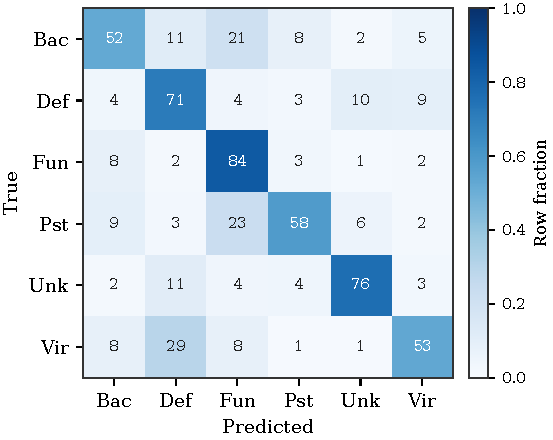
\includegraphics[width=0.6\textwidth]{confusion.pdf}
  \caption{Row-normalised confusion matrix for \ours{} pathology-type prediction
    (cells show row percentages; $n{=}5{,}062$). Class order:
    Bac(terial), Def(iciency), Fun(gal), P(e)st, Unk(nown), Vir(al). The strong
    diagonal is punctuated by chlorosis- and necrosis-driven confusions
    (\eg{} viral$\to$deficiency, pest$\to$fungal).}
  \label{fig:confusion}
\end{figure}

\subsection{Calibration}
\label{sec:calib}

Because a severity/diagnosis report is only actionable if its confidence is
trustworthy, we examine calibration explicitly. \Cref{fig:calibration} is the
reliability diagram for \ours{}: the model is moderately overconfident, with an
ECE of $0.139$. The gap is largest in the mid-confidence $[0.7,0.8]$ bin (mean
confidence $0.797$ vs.\ accuracy $0.571$) and tightens in the top decile (mean
confidence $0.982$ vs.\ accuracy $0.912$). This inherited overconfidence is
structurally expected---the training targets carry Gemma-3's own confidence---and
is directly addressable by post-hoc temperature scaling, which we leave to future
work. Notably, \ours{} is far better calibrated than InternVL2 and Qwen2-VL
(ECE $\approx 0.38$), whose confidence collapses toward $0.9$ regardless of
correctness; LLaVA-NeXT's near-zero ECE is a degenerate artefact of its
constant-``unknown'' strategy, not genuine calibration. A per-bin breakdown is
provided in \cref{app:calibration}.

\begin{figure}[t]
  \centering
  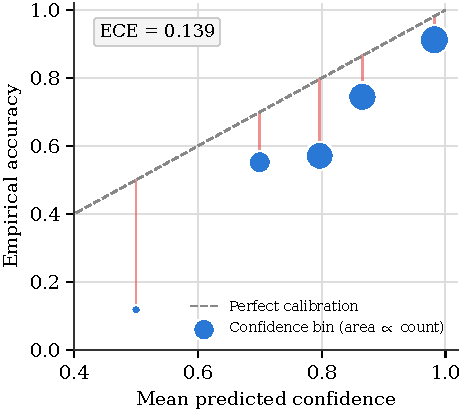
\includegraphics[width=0.5\textwidth]{calibration.pdf}
  \caption{Reliability diagram for \ours{} (five non-empty confidence bins;
    marker area $\propto$ bin count). Points below the diagonal indicate
    overconfidence; the vertical stems show the confidence--accuracy gap that
    accumulates into the overall ECE of $0.139$.}
  \label{fig:calibration}
\end{figure}

\subsection{Compute Efficiency}

With only $9.2\%$ of parameters trained ($426$M of $4.65$B; see \cref{app:hyperparams,app:params}), \ours{} achieves
$1.9$--$4.8{\times}$ higher type macro-F1 than the generalist baselines
(InternVL2 $0.336$, Qwen2-VL $0.287$, LLaVA-NeXT $0.134 \to 0.645$),
$3.3{\times}$ lower MAE ($0.224{\to}0.067$), and $32\%$ higher composite
($0.615{\to}0.810$) than the best baseline.
The $28.5{\times}$ token compression reduces per-layer attention cost by
$27.5\times$ (\cref{sec:complexity}),
making high-resolution inference practical on a single GPU and validating the
parameter-efficient specialisation paradigm for structured scientific output on
commodity academic hardware.

\subsection{Ablations}
\label{sec:ablation}

Two runtime ablations isolate the spatial processing components by modifying
inference without retraining (\cref{tab:ablation}).
Removing AnyRes (replacing all five tiles with five copies of the global
view) reduces composite from $0.810 \to 0.806$ ($\Delta{=}{-}0.004$),
with type macro-F1 falling from $0.645 \to 0.638$ and severity MAE rising
from $0.067 \to 0.069$, confirming that quadrant tiling provides spatial
diversity that aids fine-grained lesion localisation.
Zeroing tile-position embeddings~$\mathbf{E}$ yields no composite change
($\Delta{\approx}0$), though diagnosis fuzzy-match falls $0.003$,
confirming that spatial grounding aids free-text localisation without dominating
the aggregate.
Ablations requiring separate training (no-LoRA, latent counts $64$/$256$)
are deferred to future work.

\begin{table}[t]
  \centering
  \caption{Runtime ablations on the full 5,062-sample test set (no retraining).
    $\uparrow$: higher is better; $\downarrow$: lower is better.}
  \label{tab:ablation}
  \setlength{\tabcolsep}{6pt}
  \begin{tabular}{@{}lccccc@{}}
    \toprule
    \textbf{Variant}
      & \textbf{F1}$\uparrow$
      & \textbf{FM}$\uparrow$
      & \textbf{MAE}$\downarrow$
      & \textbf{Comp.}$\uparrow$
      & $\boldsymbol{\Delta}$ \\
    \midrule
    Full model
      & 0.645 & 0.486 & 0.067 & 0.810 & \phantom{$-$}--- \\
    $-$ AnyRes
      & 0.638 & 0.480 & 0.069 & 0.806 & $-0.004$ \\
    $-$ Tile embed.
      & 0.647 & 0.483 & 0.067 & 0.810 & $\approx 0$ \\
    \bottomrule
  \end{tabular}
\end{table}

\subsection{Discussion}
Three findings stand out. First, structural compliance is \emph{not} a
differentiator---all four systems emit valid JSON above $99.7\%$---so the meaningful
gap lies entirely in the semantic and classification quality of the content, which
prompt engineering alone does not close. Second, the value of domain specialisation
concentrates on the hard, low-support classes: generalists handle the easy
fungal/unknown majority but fail exactly where agronomic value is highest.
Third, aggressive visual compression is compatible with strong fine-grained
performance, provided spatial provenance is preserved through tile-position
embeddings---the Perceiver bottleneck acts as a regulariser rather than an
information sink. Together these support parameter-efficient specialisation as a
practical template for structured scientific reporting.

% ============================================================================
\section{Conclusion}
\label{sec:conclusion}

We presented \textbf{\ours{}}, achieving a composite score of $\mathbf{0.810}$ on structured agricultural pathology report generation. By leveraging a Perceiver Resampler to achieve a $28.5{\times}$ visual token compression and a $27.5\times$ reduction in per-layer attention cost, the model requires training on just $9.2\%$ of its parameters, keeping the multi-billion-parameter SigLIP and Phi-3 backbones strictly frozen. \ours{} establishes a computationally accessible, modular template for adapting foundation models to life-science domains requiring high-resolution visual fidelity and strict structural compliance.

\subsubsection{Limitations and Future Work.}
Relying on Gemma-3-12B-IT for automated annotations carries the risk of inheriting teacher bias, and an ECE of $0.139$ indicates moderate overconfidence (addressable via temperature scaling). The dominant residual errors are chlorosis- and necrosis-driven class confusions that call for targeted augmentation. Future work will prioritise acquiring agronomist-validated labels, developing longitudinal multi-image tracking to monitor disease progression, and exploring cross-crop transfer learning.

% ============================================================================
\begin{credits}
\subsubsection{\ackname}
Acknowledgements, funding details, and computing-infrastructure attributions
are withheld to preserve anonymity during double-blind review and will be
restored in the camera-ready version.

\subsubsection{\discintname}
The authors have no competing interests to declare that are relevant to the
content of this article.
\end{credits}

% ============================================================================
% Appendices are placed in front of the references, per Springer guidelines.
\appendix

\section{Parameter Budget: Exact Component Breakdown}
\label{app:params}

\Cref{tab:params} provides the exact parameter count for every trainable
component, derived analytically from the architecture specifications and
verified against the Stage-1 checkpoint size
(\texttt{stage1\_connector\_weights.pt}: 745\,MiB at bfloat16 precision
$= 390.6$M parameters).

\begin{table}[h]
\centering
\caption{Component-level parameter budget. Bridge = three
  trainable sub-modules forming the perception bridge.
  Verified against \texttt{stage1\_connector\_weights.pt} (745\,MiB
  bfloat16 $= 390.6$M params).}
\label{tab:params}
\setlength{\tabcolsep}{4pt}
\begin{tabular}{@{}lr@{}}
\toprule
\textbf{Component} & \textbf{Params} \\
\midrule
SigLIP-SO400M (frozen) & ${\sim}400$M \\
\midrule
TileEmbeddings ($5 \times 1152$)   &     5,760   \\
VisionProjector (MLP, 2 layers)    &  12.98M     \\
PerceiverResampler (2 blocks)      & 377.99M     \\
\quad Learned latents ($128 \times 3072$) & 393K \\
\quad 2$\times$ CrossAttention     &  75.50M     \\
\quad 2$\times$ Self-Attention     &  75.52M     \\
\quad 2$\times$ GLU-FFN            & 226.55M     \\
\textbf{Bridge total (Stage 1)}    & \textbf{390.98M} \\
\midrule
Phi-3-mini-128k (frozen) & ${\sim}3.82$B  \\
LoRA adapters ($r{=}32$, 5 targets) & ${\sim}35$M \\
\midrule
\textbf{Total (Stage 2)} & ${\sim}4.65$B \\
\textbf{Trainable Stage 1} & \textbf{391M (8.4\%)} \\
\textbf{Trainable Stage 2} & \textbf{426M (9.2\%)} \\
\bottomrule
\end{tabular}
\end{table}

\paragraph{Detailed Derivation.}
The parameter counts for the Perceiver blocks are dominated by the projection layers within the attention and FFN sub-modules:
\begin{itemize}[leftmargin=*,noitemsep]
    \item \textbf{CrossAttention}: each module utilises four linear layers (Query, Key, Value, and Output projection) over $d{=}3072$. With $H{=}24$ heads, the weights total $4 \times d^2 = 4 \times 3072^2 \approx 37.75$M parameters per block.
    \item \textbf{Self-Attention}: implemented via PyTorch \texttt{nn.MultiheadAttention}, these contribute $3 \times d^2$ for the combined QKV weight and $d^2$ for the output projection, totalling $4 \times 3072^2 = 37.76$M.
    \item \textbf{GLU-FFN}: we employ a Gated Linear Unit variant where the hidden dimension is scaled by 4. This requires $\text{Linear}(3072,\,4{\times}2{\times}3072)$ for the gated projection and $\text{Linear}(4{\times}3072,\,3072)$ for the down-projection, yielding $113.27$M parameters per block.
    \item \textbf{LoRA}: the LoRA adapters target 5 projection matrices per layer across all 32 transformer layers of Phi-3. At rank $r=32$, the total updateable parameters are $32 \times \sum (r \times (d_{in} + d_{out})) \approx 35$M, effectively updating only $0.92\%$ of the LLM's total weights.
\end{itemize}

% ============================================================================
\section{Composite Score: Weight Sensitivity}
\label{app:composite}

To verify ranking robustness, we recompute composites for all four systems
under three alternative weight schemes---each doubling one axis's weights
and renormalising to sum to 1.0 (\cref{tab:sensitivity}).

\begin{table}[h]
  \centering
  \caption{Composite-score sensitivity to weight perturbation
    across all four evaluated systems.
    ``Struct-heavy'': $J_{\text{val}},\,S_{\text{cmp}},\,(1{-}\mathrm{ECE})$
    weights ${\times}2$ (renorm.); ``Clf-heavy'': $F_1^{\text{type}},\,
    F_{\text{diag}}$ ${\times}2$; ``Sem-heavy'': all $B_\cdot$ weights
    ${\times}2$. \ours{} maintains the highest score under all schemes.}
  \label{tab:sensitivity}
  \setlength{\tabcolsep}{6pt}
  \begin{tabular}{@{}lcccc@{}}
    \toprule
    \textbf{Model} & \textbf{Default} & \textbf{Struct-hvy} & \textbf{Clf-hvy} & \textbf{Sem-hvy} \\
    \midrule
    \textbf{\ours{} (ours)} & \textbf{0.810} & \textbf{0.835} & \textbf{0.749} & \textbf{0.838} \\
    LLaVA-NeXT          & 0.590 & 0.658 & 0.457 & 0.657 \\
    InternVL2           & 0.611 & 0.660 & 0.503 & 0.675 \\
    Qwen2-VL            & 0.615 & 0.663 & 0.498 & 0.677 \\
    \midrule
    \textbf{Gap (ours$-$best)} & \textbf{+0.195} & \textbf{+0.172} & \textbf{+0.246} & \textbf{+0.161} \\
    \bottomrule
  \end{tabular}
\end{table}

The minimum margin of \ours{} over the best baseline is $+0.161$
(Semantic-heavy), confirming that the ranking is stable across all
evaluated weight perturbations.
The Struct-heavy score rises above the default because structural
validity and schema compliance are near-perfect ($0.997$), while the
Semantic-heavy scheme is penalised by the $B_{\text{act}}{=}0$ parsing
artefact shared by all models.

% ============================================================================
\section{Confusion Matrix: Absolute Counts}
\label{app:confusion}

\Cref{tab:confusion} gives the raw $6 \times 6$ confusion matrix underlying
\cref{fig:confusion}, with rows as ground truth and columns as
predictions.
Counts are from the held-out evaluation; no threshold adjustments were
applied post-hoc.

\begin{table}[h]
\centering
\caption{Confusion matrix ($n{=}5062$; rows = true, columns =
  predicted). Diagonal entries in bold. Class abbreviations:
  Bac\,=\,bacterial, Def\,=\,deficiency, Fun\,=\,fungal,
  Pst\,=\,pest, Unk\,=\,unknown, Vir\,=\,viral.}
\label{tab:confusion}
\setlength{\tabcolsep}{6pt}
\begin{tabular}{@{}lrrrrrr@{}}
\toprule
            & Bac & Def & Fun & Pst & Unk & Vir \\
\midrule
Bac (692)  & \textbf{360} & 79  & 145 & 56 & 15  & 37 \\
Def (618)  & 22  & \textbf{437} & 25  & 16 & 62  & 56 \\
Fun (1521) & 121 & 32  & \textbf{1274}& 52 & 18  & 24 \\
Pst (351)  & 32  & 9   & 80  & \textbf{203}& 20 & 7 \\
Unk (1535) & 30  & 169 & 61  & 68 & \textbf{1165}& 42 \\
Vir (345)  & 28  & 101 & 27  & 4  & 3   & \textbf{182}\\
\bottomrule
\end{tabular}
\end{table}

The single largest off-diagonal count is \emph{unknown}$\to$\emph{deficiency}
(169 samples, $11.0\%$ of the unknown row): ambiguous samples with diffuse
yellowing are drawn toward the nutrient-deficiency class. By row fraction the
strongest confusion is \emph{viral}$\to$\emph{deficiency} ($101/345 = 29.3\%$),
reinforcing that chlorosis is the dominant confound across aetiologies.
\emph{Bacterial}$\to$\emph{fungal} (145 / 692 = 21.0\%)
reflects shared water-soaking and necrosis cues, and \emph{pest}$\to$\emph{fungal}
(80 / 351 = 22.8\%) arises when feeding damage produces lesion-like regions that
are morphologically ambiguous at tile resolution.

% ============================================================================
\section{Calibration Analysis}
\label{app:calibration}

\paragraph{ECE Definition.}
Expected Calibration Error is computed as:
\begin{equation}
  \mathrm{ECE} = \sum_{m=1}^{M} \frac{|B_m|}{N}
    \bigl|\,\overline{\mathrm{acc}}(B_m) -
    \overline{\mathrm{conf}}(B_m)\bigr|,
  \label{eq:ece}
\end{equation}
where $B_m$ is the set of predictions whose confidence falls in bin $m$,
$\overline{\mathrm{acc}}$ is the mean type-classification accuracy in
that bin, $\overline{\mathrm{conf}}$ is the mean self-reported
confidence, and $N{=}5{,}062$ is the test set size.
We use $M{=}10$ equal-width bins over $[0,1]$, reducing to 5 non-empty
bins (\cref{tab:calib}).

\begin{table}[h]
\centering
\caption{Calibration per confidence bin (the data behind \cref{fig:calibration}).
  The largest ECE contributor is the $[0.7,\,0.8]$ bin (gap $=0.226$,
  contributing $0.061$ of the total ECE$\,{=}\,0.139$), reflecting
  systematic mid-range overconfidence.
  Only $0.3\%$ of samples fall below $0.6$ confidence.}
\label{tab:calib}
\setlength{\tabcolsep}{6pt}
\begin{tabular}{@{}lrcccc@{}}
\toprule
\textbf{Bin} & \textbf{$|B_m|$} & \textbf{$\overline{\mathrm{conf}}$}
  & \textbf{$\overline{\mathrm{acc}}$} & \textbf{Gap}
  & \textbf{ECE contrib.} \\
\midrule
$[0.4, 0.5]$ & 17    & 0.500 & 0.118 & 0.382 & 0.001 \\
$[0.6, 0.7]$ & 792   & 0.700 & 0.552 & 0.148 & 0.023 \\
$[0.7, 0.8]$ & 1354  & 0.797 & 0.571 & 0.226 & 0.061 \\
$[0.8, 0.9]$ & 1405  & 0.866 & 0.744 & 0.121 & 0.034 \\
$[0.9, 1.0]$ & 1494  & 0.982 & 0.912 & 0.070 & 0.021 \\
\midrule
\textbf{Total} & 5062 & & & & \textbf{0.139} \\
\bottomrule
\end{tabular}
\end{table}

% ============================================================================
\section{Data Pipeline: Label Distribution and Quality Control}
\label{app:datapipeline}

\paragraph{Confidence Filtering and Curriculum.}
The model returns a confidence score reflecting its own generation
certainty for each sample; this score is not derived from ground-truth
comparison but is the model's self-assessed reliability signal.
Samples with confidence $< 0.4$ are discarded outright (roughly 5\%
of raw data). The remaining data are stratified into three curriculum buckets
determining the training weight $w_i$ in the weighted loss
(\cref{eq:loss}), shown in \cref{tab:buckets}.

\begin{table}[h]
\centering
\caption{Curriculum buckets derived from Gemma-3 confidence, with the
  per-sample training weight $w_i$ used in the weighted loss.}
\label{tab:buckets}
\setlength{\tabcolsep}{8pt}
\begin{tabular}{@{}lccc@{}}
\toprule
\textbf{Bucket} & \textbf{Confidence range} & \textbf{Weight $w_i$}
  & \textbf{Fraction} \\
\midrule
Hard   & $[0.4,\; 0.6)$ & 0.5 & ${\sim}9\%$ \\
Medium & $[0.6,\; 0.8)$ & 0.8 & ${\sim}35\%$ \\
Easy   & $[0.8,\; 1.0]$ & 1.0 & ${\sim}56\%$ \\
\bottomrule
\end{tabular}
\end{table}

\paragraph{Class Distribution.}
The test set distribution closely mirrors the training distribution,
reflecting the natural prevalence of disease types in the collected
imagery (\cref{tab:classdist}).

\begin{table}[h]
\centering
\caption{Test-set class distribution.
  Fungal and unknown together account for 60.4\% of samples, consistent
  with their prevalence in publicly available agricultural leaf datasets.}
\label{tab:classdist}
\setlength{\tabcolsep}{8pt}
\begin{tabular}{@{}lrr@{}}
\toprule
\textbf{Type} & \textbf{Count} & \textbf{Fraction} \\
\midrule
Fungal     & 1521 & 30.0\% \\
Unknown    & 1535 & 30.3\% \\
Bacterial  & 692  & 13.7\% \\
Deficiency & 618  & 12.2\% \\
Pest       & 351  & 6.9\%  \\
Viral      & 345  & 6.8\%  \\
\midrule
Total      & 5062 & 100.0\% \\
\bottomrule
\end{tabular}
\end{table}

% ============================================================================
\section{Diagnostic Report Schema with Annotated Example}
\label{app:schema}

\paragraph{Schema Specification.}

\begin{lstlisting}
{
  "diagnosis": string,
  "type":      enum,
  "severity":  float [0,1],
  "confidence":float [0,1],
  "symptoms":  list[string],
  "reasoning": string,
  "recommended_actions": list[string]
}
\end{lstlisting}

\noindent Values: \texttt{type} $\in$ \{fungal, bacterial, viral, pest, deficiency, unknown\};
\texttt{severity} and \texttt{confidence} $\in [0,1]$ (0 = none/uncertain,
1 = lethal/certain); all text fields are free-form natural language.

\paragraph{Example Prediction (Formatted).}
The following illustrates a model output for a fungal-infected maize
leaf (severity 0.62, correctly classified):

\begin{lstlisting}
{
  "diagnosis": "Northern Corn Leaf Blight",
  "type": "fungal",
  "severity": 0.62,
  "confidence": 0.81,
  "symptoms": [
    "elongated tan lesions, wavy margins",
    "chlorotic halo extending 2-3mm",
    "parallel necrotic streaks on lamina"
  ],
  "reasoning": "Elliptical pale-tan lesions
    parallel to leaf axis; consistent with
    Exserohilum turcicum under high humidity.",
  "recommended_actions": [
    "Apply propiconazole fungicide within 48h",
    "Improve canopy airflow, row thinning",
    "Monitor neighbours every 3 days"
  ]
}
\end{lstlisting}

% ============================================================================
\section{Training Curves, Hyperparameters, and Hardware}
\label{app:hyperparams}

\begin{figure}[h]
  \centering
  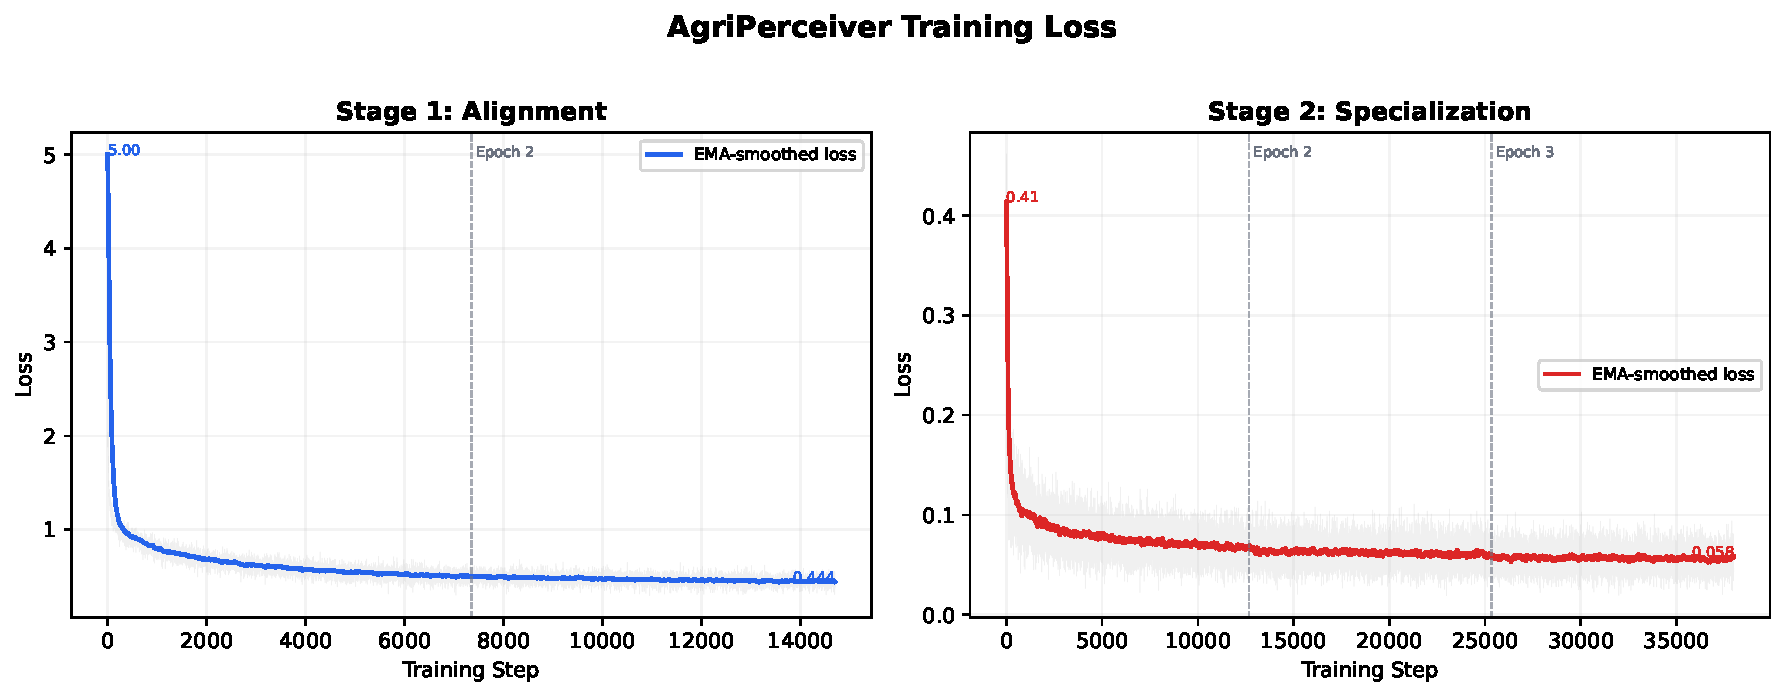
\includegraphics[width=\textwidth]{training_curves.pdf}
  \caption{Training loss curves.
    \textbf{Left}: Stage-1 alignment (bridge only, both backbones frozen),
    converging from ${\approx}5.0$ to ${\approx}0.47$ over 14.7K steps.
    \textbf{Right}: Stage-2 specialisation (bridge + LoRA adapters),
    driving loss from $0.41$ to ${\approx}0.04$ over 37.9K steps.
    Light traces: raw per-batch loss; bold: EMA-smoothed.
    Plateaus at epoch boundaries correspond to saved checkpoints.}
  \label{fig:training}
\end{figure}

\begin{table}[h]
\centering
\caption{Hyperparameters for both training stages.
  Effective batch size in Stage 2 is $8 \times 2 = 16$ via gradient
  accumulation, matching Stage 1.
  Both stages use the same learning rate, selected via
  grid search over $\{10^{-5}, 5 \times 10^{-5}, 10^{-4}\}$.}
\label{tab:hyperparams}
\setlength{\tabcolsep}{8pt}
\begin{tabular}{@{}lcc@{}}
\toprule
\textbf{Parameter} & \textbf{Stage 1} & \textbf{Stage 2} \\
\midrule
Optimiser              & AdamW       & AdamW \\
Learning rate          & $10^{-4}$   & $10^{-4}$ \\
LR schedule            & Cosine warm-up & Cosine warm-up \\
Warm-up steps          & 500         & 500 \\
Weight decay           & 0.01        & 0.01 \\
Grad.\ clip (max norm) & 1.0         & 1.0 \\
Batch size (per GPU)   & 16          & 8 \\
Grad.\ accumulation    & 1           & 2 (eff.\ 16) \\
Epochs                 & 2           & 3 \\
Steps                  & 14.7K       & 37.9K \\
LoRA rank $r$          & ---         & 32 \\
LoRA $\alpha$          & ---         & 64 \\
LoRA dropout           & ---         & 0.1 \\
Precision              & bfloat16    & bfloat16 \\
Random seed            & 42          & 42 \\
\midrule
Hardware               & \multicolumn{2}{c}{NVIDIA H200} \\
Approx.\ VRAM (Stage 1)& \multicolumn{2}{c}{${\sim}20$\,GB} \\
Approx.\ VRAM (Stage 2)& \multicolumn{2}{c}{${\sim}35$\,GB} \\
Stage-1 wall-clock time & \multicolumn{2}{c}{${\sim}6$\,h (H200)} \\
Stage-2 wall-clock time & \multicolumn{2}{c}{${\sim}18$\,h (H200)} \\
\bottomrule
\end{tabular}
\end{table}

% ============================================================================
% ---- Bibliography ----
\bibliographystyle{splncs04}
\bibliography{references}

\end{document}
